\qns{Bode Plots for Filters}
\qcontributor{Ramsey Mardini}
\qcontributor{Naomi Sagan}
\qcontributor{Ryan Koh}

\begin{enumerate}

\qitem First, consider the following transfer function of a Low-Pass Filter: $H(\omega) = \frac{1}{j\omega C_{1}R_{1} + 1}$ where $R_{1} = 100 \Omega$ and $C_{1} = 100 pF$
    \begin{enumerate}
        \qitem What is its cutoff frequency?

        \sol{
        $\omega_{c} = \frac{1}{R_{1}C_{1}} = \frac{1}{10^{2} \cdot 10^{-10}} = 10^{8}$
        }
        \qitem Sketch its phase and magnitude.

        \sol{
        Magnitude (log-log scale): According to our Bode plot approximation, the magnitude of $H(\omega)$ is 1 until $\omega_{c}$, after which it decreases linearly with a slope of 1.
        \newline
        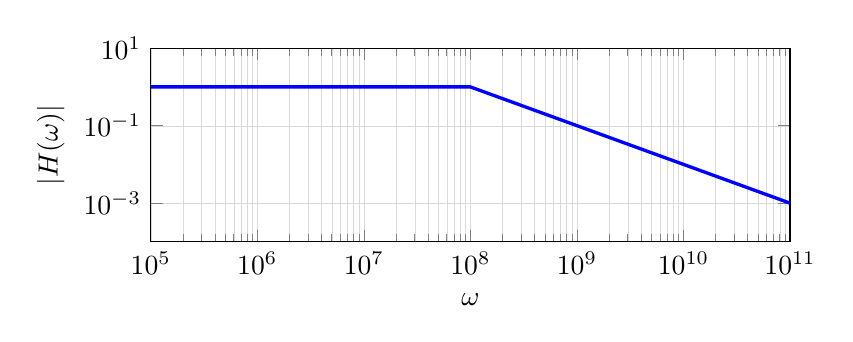
\begin{tikzpicture}[
          declare function={
            mag(\omega)= (\omega < 10^8) * (1) +
                      (\omega >= 10^8) * (10^8 / \omega)
           ;
          }
        ]
          \begin{loglogaxis}[
            ymin=0.0001, ymax=10, ylabel=$|H(\omega)|$,
            xmin=10^5, xmax=10^11, xlabel=$\omega$,
            domain=10^5:10^11,
            grid=both, grid style={line width=.1pt, draw=gray!30},
            width=\textwidth * 0.8,
            height=\textwidth / 3
          ]
            \addplot [blue,very thick] {mag(x)};
          \end{loglogaxis}
        \end{tikzpicture}
        
        Phase (semi-log scale): According to our Bode plot approximation, the phase of $H(\omega)$ is 0 until $\frac{\omega_{c}}{10}$, after which it decreases linearly until $10\omega_{c}$, where it stays at $-\frac{\pi}{2}$.
        At $\omega_{c}$, the phase is exactly $-\frac{\pi}{4}$.
        \newline
        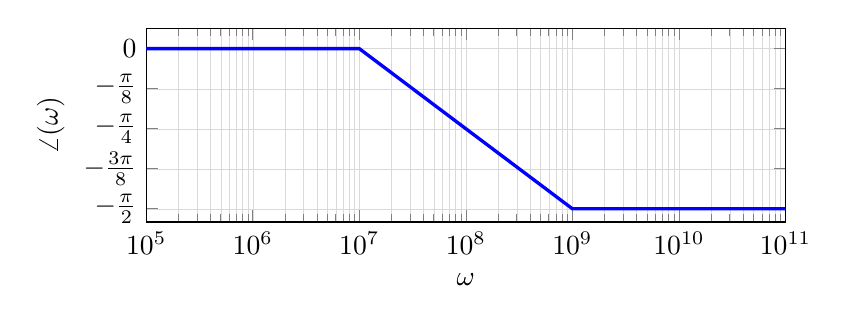
\begin{tikzpicture}[
          declare function={
            phase(\omega)= (\omega < 10^7) * (0) +
                      and(\omega >= 10^7, \omega < 10^9) * (-pi / 4 * (log10(\omega) - 7)) +
                      (\omega >= 10^9) * (-pi / 2)
           ;
          }
        ]
          \begin{semilogxaxis}[
            ymin= -1.7, ymax=0.2, ylabel=$\angle(\omega)$,
            ytick={-pi/2, -3*pi/8, -pi/4, -pi/8, 0},
            yticklabels={$-\frac{\pi}{2}$,$-\frac{3\pi}{8}$,$-\frac{\pi}{4}$,$-\frac{\pi}{8}$,$0$},
            xmin=10^5, xmax=10^11, xlabel=$\omega$,
            domain=10^5:10^11,
            grid=both, grid style={line width=.1pt, draw=gray!30},
            width=\textwidth * 0.8,
            height=\textwidth / 3
          ]
            \addplot [blue,very thick] {phase(x)};
          \end{semilogxaxis}
        \end{tikzpicture}
        }
        \newline
        \meta{
        \newline
        Intuition behind the magnitude bode plot approximation: until $\omega_{c}$, the $1$ term in the denominator is larger than the $\frac{j\omega}{\omega_{c}}$ term, so $1 + \frac{j\omega}{\omega_{c}}$ can be approximated as $1$, so the entire transfer function is approximated as $1$.
        After $\omega_{c}$, the $\frac{j\omega}{\omega_{c}}$ term in the denominator is larger, so the transfer function can be approximated as $\frac{1}{\frac{j\omega}{\omega_{c}}}$, or $\frac{\omega_{c}}{j\omega}$. \\
        Intuition behind the phase bode plot approximation: The phase of $H(\omega)$ is $\angle(numerator) - \angle(denominator) = 0 - \angle(1 + \frac{j\omega}{\omega_{c}})$.
        We approximate this as being equal to $-\angle(1)$, or $0$, until $\frac{\omega_{c}}{10}$ and $-\angle(\frac{j\omega}{\omega_{c}})$, or $-\frac{\pi}{2}$, after $10 \omega_{c}$.
        Between $\frac{\omega_{c}}{10}$ and $10 \omega_{c}$, we approximate the phase with a straight line. \\
        The same ideas apply to part (b).
        }
    \end{enumerate}

\qitem Now consider the transfer function of a High-Pass Filter: $H(\omega) = \frac{j\omega C_{2}R_{2}}{j\omega C_{2}R_{2} + 1}$ where $R_{2} = 1 k\Omega$ and $C_{1} = 10 nF$
    \begin{enumerate}
        \qitem What is its cutoff frequency?

        \sol{
        $\omega_{c} = \frac{1}{R_{2}C_{2}} = \frac{1}{10^{3} \cdot 10^{-8}} = 10^{5}$
        }
        \qitem Sketch its phase and magnitude.

        \sol{
        Magnitude (log-log scale): According to our Bode plot approximation, the magnitude of $H(\omega)$ increases linearly with a slope of 1 until $\omega_{c}$, after which it levels off at 1.
        \newline
        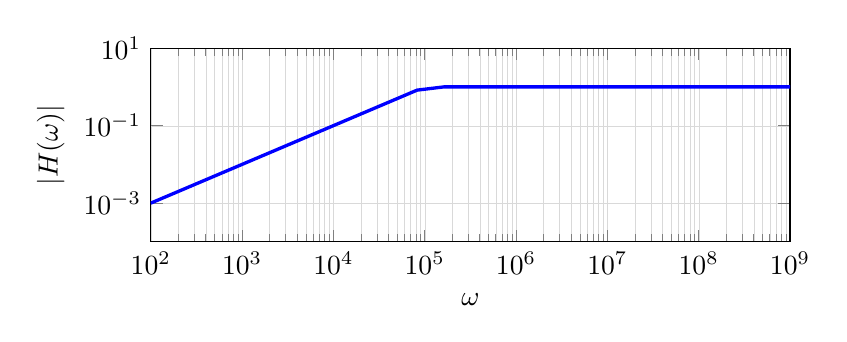
\begin{tikzpicture}[
          declare function={
            mag(\omega)= (\omega < 10^5) * (\omega / 10^5) +
                      (\omega >= 10^5) * (1)
           ;
          }
        ]
          \begin{loglogaxis}[
            ymin=0.0001, ymax=10, ylabel=$|H(\omega)|$,
            xmin=10^2, xmax=10^9, xlabel=$\omega$,
            domain=10^2:10^9,
            grid=both, grid style={line width=.1pt, draw=gray!30},
            width=\textwidth * 0.8,
            height=\textwidth / 3
          ]
            \addplot [blue,very thick] {mag(x)};
          \end{loglogaxis}
        \end{tikzpicture}
        
        Phase (semi-log scale): According to our Bode plot approximation, the phase of $H(\omega)$ is $\frac{\pi}{2}$ until $\frac{\omega_{c}}{10}$, after which it decreases linearly until $10\omega_{c}$, where it stays at $0$.
        At $\omega_{c}$, the phase is  $-\frac{\pi}{4}$.
        \newline
        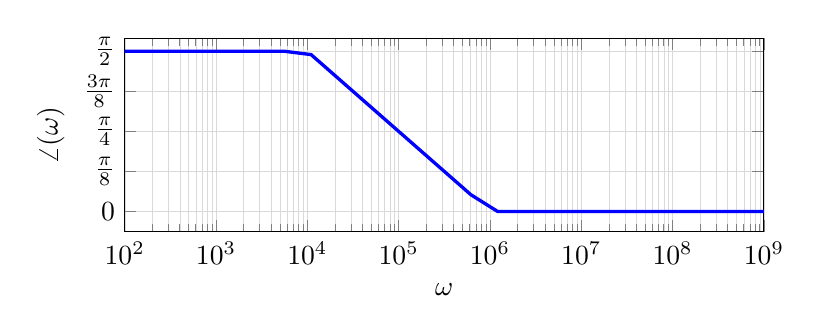
\begin{tikzpicture}[
          declare function={
            phase(\omega)= (\omega < 10^4) * (pi / 2) +
                      and(\omega >= 10^4, \omega < 10^6) * (-pi / 4 * (log10(\omega) - 4) + pi / 2) +
                      (\omega >= 10^6) * (0)
           ;
          }
        ]
          \begin{semilogxaxis}[
            ymin= -0.2, ymax=1.7, ylabel=$\angle(\omega)$,
            ytick={pi/2, 3*pi/8, pi/4, pi/8, 0},
            yticklabels={$\frac{\pi}{2}$,$\frac{3\pi}{8}$,$\frac{\pi}{4}$,$\frac{\pi}{8}$,$0$},
            xmin=10^2, xmax=10^9, xlabel=$\omega$,
            domain=10^2:10^9,
            grid=both, grid style={line width=.1pt, draw=gray!30},
            width=\textwidth * 0.8,
            height=\textwidth / 3
          ]
            \addplot [blue,very thick] {phase(x)};
          \end{semilogxaxis}
        \end{tikzpicture}
        }
    \end{enumerate}

\qitem What happens if we cascade these two filters together with a unity-gain buffer in between them? Consider the resulting transfer function: 
        $H(\omega) = \frac{1}{j\omega C_{1}R_{1} + 1} \cdot \frac{j\omega C_{2}R_{2}}{j\omega C_{2}R_{2} + 1}$
    \begin{enumerate}
        \qitem What are its cutoff frequencies?

        \sol{
        The lower cutoff is the cutoff frequency of the high-pass filter:
        $$\omega_{c,l} = \frac{1}{R_{2}C_{2}} = 10^{5}$$
        The upper cutoff is the cutoff frequency of the low-pass filter:
        $$\omega_{c,u} = \frac{1}{R_{1}C_{1}} = 10^{8}$$
        }
        \qitem Sketch its phase and magnitude. \textit{Hint: How can we combine the plots of the individual filters together?}

        \sol{
        For both the magnitude and the phase plots, you can "add" the high-pass filter to the low-pass filter.
        \newline
        \newline
        Magnitude plot:
        \newline
        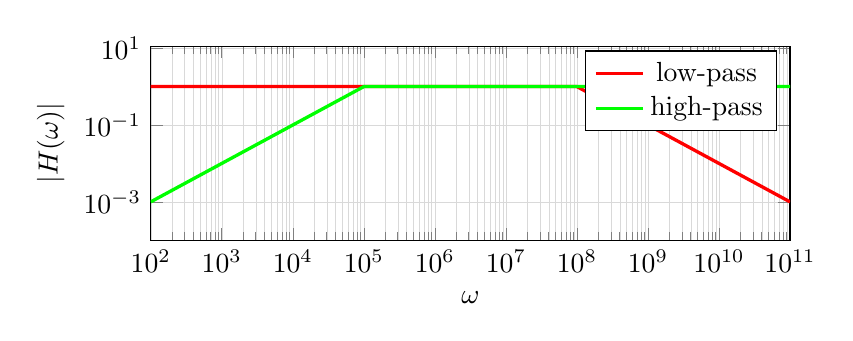
\begin{tikzpicture}[
          declare function={
            highpass(\omega)= (\omega < 10^5) * (\omega / 10^5) +
                      (\omega >= 10^5) * (1)
           ;
           lowpass(\omega)= (\omega < 10^8) * (1) +
                     (\omega >= 10^8) * (10^8 / \omega)
          ;
          }
        ]
          \begin{loglogaxis}[
            ymin=0.0001, ymax=11, ylabel=$|H(\omega)|$,
            xmin=10^2, xmax=10^11, xlabel=$\omega$,
            domain=10^2:10^11,
            grid=both, grid style={line width=.1pt, draw=gray!30},
            width=\textwidth * 0.8,
            height=\textwidth / 3
          ]
            \addplot [red,very thick] {lowpass(x)};
            \addlegendentry{low-pass}
            \addplot [green,very thick] {highpass(x)};
            \addlegendentry{high-pass}
          \end{loglogaxis}
        \end{tikzpicture}
        \newline
        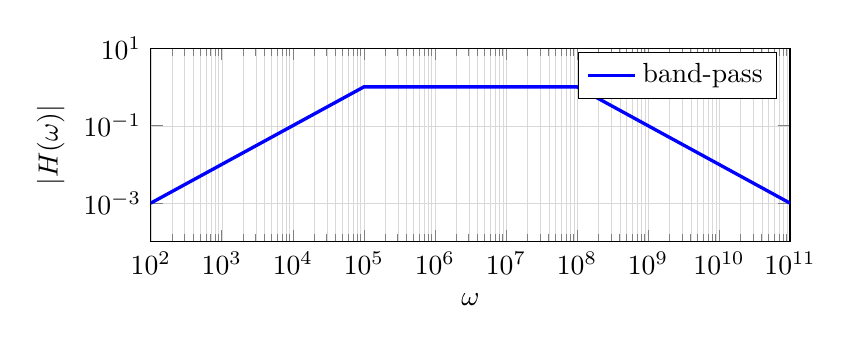
\begin{tikzpicture}[
          declare function={
            highpass(\omega)= (\omega < 10^5) * (\omega / 10^5) +
                      (\omega >= 10^5) * (1)
           ;
           lowpass(\omega)= (\omega < 10^8) * (1) +
                     (\omega >= 10^8) * (10^8 / \omega)
          ;
          }
        ]
          \begin{loglogaxis}[
            ymin=0.0001, ymax=10, ylabel=$|H(\omega)|$,
            xmin=10^2, xmax=10^11, xlabel=$\omega$,
            domain=10^2:10^11,
            grid=both, grid style={line width=.1pt, draw=gray!30},
            width=\textwidth * 0.8,
            height=\textwidth / 3
          ]
            \addplot [blue,very thick] {lowpass(x) * highpass(x)};
            \addlegendentry{band-pass}
            
          \end{loglogaxis}
        \end{tikzpicture}
        \newline
        Phase plot:
        \newline
        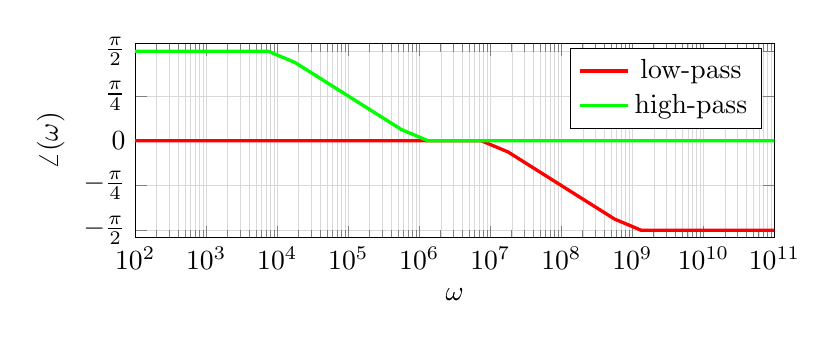
\begin{tikzpicture}[
          declare function={
            lowpass(\omega)= (\omega < 10^7) * (0) +
                      and(\omega >= 10^7, \omega < 10^9) * (-pi / 4 * (log10(\omega) - 7)) +
                      (\omega >= 10^9) * (-pi / 2)
           ;
           highpass(\omega)= (\omega < 10^4) * (pi / 2) +
                     and(\omega >= 10^4, \omega < 10^6) * (-pi / 4 * (log10(\omega) - 4) + pi / 2) +
                     (\omega >= 10^6) * (0)
          ;
          }
        ]
          \begin{semilogxaxis}[
            ymin= -1.7, ymax=1.7, ylabel=$\angle(\omega)$,
            ytick={-pi/2, -pi/4, 0, pi/4, pi/2},
            yticklabels={$-\frac{\pi}{2}$,$-\frac{\pi}{4}$,$0$,$\frac{\pi}{4}$,$\frac{\pi}{2}$},
            xmin=10^2, xmax=10^11, xlabel=$\omega$,
            domain=10^2:10^11,
            grid=both, grid style={line width=.1pt, draw=gray!30},
            width=\textwidth * 0.8,
            height=\textwidth / 3
          ]
            \addplot [red,very thick] {lowpass(x)};
            \addlegendentry{low-pass}
            \addplot [green,very thick] {highpass(x)};
            \addlegendentry{high-pass}
          \end{semilogxaxis}
        \end{tikzpicture}
        \newline
        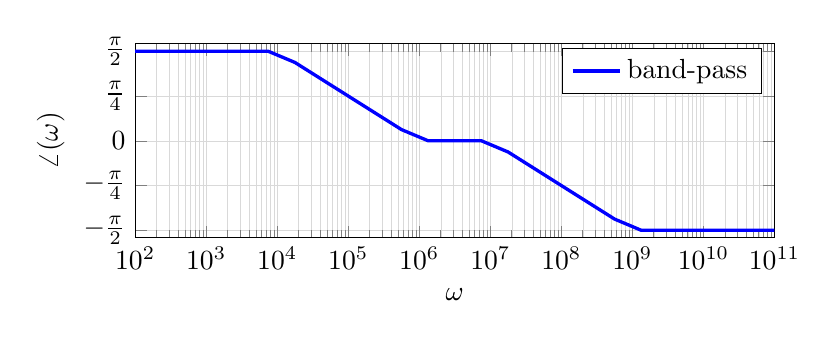
\begin{tikzpicture}[
          declare function={
            lowpass(\omega)= (\omega < 10^7) * (0) +
                      and(\omega >= 10^7, \omega < 10^9) * (-pi / 4 * (log10(\omega) - 7)) +
                      (\omega >= 10^9) * (-pi / 2)
           ;
           highpass(\omega)= (\omega < 10^4) * (pi / 2) +
                     and(\omega >= 10^4, \omega < 10^6) * (-pi / 4 * (log10(\omega) - 4) + pi / 2) +
                     (\omega >= 10^6) * (0)
          ;
          }
        ]
          \begin{semilogxaxis}[
            ymin= -1.7, ymax=1.7, ylabel=$\angle(\omega)$,
            ytick={-pi/2, -pi/4, 0, pi/4, pi/2},
            yticklabels={$-\frac{\pi}{2}$,$-\frac{\pi}{4}$,$0$,$\frac{\pi}{4}$,$\frac{\pi}{2}$},
            xmin=10^2, xmax=10^11, xlabel=$\omega$,
            domain=10^2:10^11,
            grid=both, grid style={line width=.1pt, draw=gray!30},
            width=\textwidth * 0.8,
            height=\textwidth / 3
          ]
            \addplot [blue,very thick] {lowpass(x) + highpass(x)};
            \addlegendentry{band-pass}
          \end{semilogxaxis}
        \end{tikzpicture}
        }
        \newline
        \meta{
        We can "add" the magnitudes of the high-pass and low-pass filters together because we are graphing $log(|H(\omega)|) = log(|H_{high}(\omega)| \cdot |H_{low}(\omega)|) = log(|H_{high}(\omega)|) + log(|H_{low}(\omega)|)$.
        We can "add" the phases because $\angle(H_{high}(\omega) * H_{low}(\omega)) = \angle(H_{high}(\omega)) + \angle(H_{low}(\omega))$.
        }
    \end{enumerate}
Now lets take a look at two more concepts, \textbf{bandwidth} and \textbf{Q-factor}. The bandwidth of a resonance
circuit is the difference between its upper and lower cutoff frequencies. It can also be expressed as \textit{resonance frequency} divided by its \textit{Q-factor}:

\begin{align}
    bandwidth = \Delta \omega = f_{high} - f_{low} = \frac{\omega_n}{Q}
\end{align}

The Q-factor, or quality factor, of a circuit is the ratio of power stored to power dissipated, but can also be more simply thought of as the measure of how good a circuit is,
where a higher Q-factor is often more desirable. This can be expressed mathematically as:

\begin{align}
    Q = \frac{\omega_{n}}{\Delta \omega}
\end{align}

\meta{
Circuits that have low bandwidths relative to their center frequency will have higher Q-factors.
}

    \begin{enumerate}[resume]
        \qitem Find its bandwidth.

        \sol{
        $$\Delta \omega = \omega_{c,u} - \omega_{c,l} = \frac{1}{R_{1}C_{1}} - \frac{1}{R_{2}C_{2}}$$
        $$\Delta \omega = 10^{8} - 10^{5} = 9.99 \cdot 10^{7}$$
        }
        \qitem What is its Q-factor? I.e.: $\frac{\omega_{n}}{\Delta \omega}$, where $\omega_{n}$ is the center frequency of the band.
        
        \sol{
        \newline
        Symbolically:
        $$Q = \frac{\omega_{n}}{\Delta \omega} = \frac{1/2 \cdot (\frac{1}{R_{1}C_{1}} + \frac{1}{R_{2}C_{2}})}{\frac{1}{R_{1}C_{1}} - \frac{1}{R_{2}C_{2}}}$$
        $$Q = \frac{(R_{2}C_{2} + R_{1}C_{1})}{2 \cdot (R_{2}C_{2} - R_{1}C_{1})}$$
        Numerically:
        $$Q = \frac{\omega_{n}}{\Delta \omega} = \frac{1/2 (10^{8} + 10^{5})}{9.99 \cdot 10^{7}} = \frac{5.005 \cdot 10^{7}}{9.99 \cdot 10^{7}}$$
        $$Q \approx 0.501$$
        }
    \end{enumerate}
\end{enumerate} 
